%!TEX program = xelatex 
\documentclass{standalone}%opcao draft remove os links
\usepackage{amssymb,amsmath,amsfonts,amsthm,amstext,pxfonts}
\usepackage{graphicx}
\usepackage[usenames,dvipsnames]{xcolor}
\usepackage{subfigure}
\usepackage{tikz,tikz-3dplot,tkz-euclide,circuitikz,siunitx,pstricks-add,pst-coil,pst-3dplot}
\usepackage{pst-plot,pst-func,pst-eucl,pst-solides3d}
\usetkzobj{all}
\usetikzlibrary{scopes}
\usetikzlibrary{through}
\usetikzlibrary{lindenmayersystems}
\usetikzlibrary[shadings]
\usetikzlibrary{arrows}
\usetikzlibrary{intersections,positioning}


\begin{document}
    \pagenumbering{gobble}
    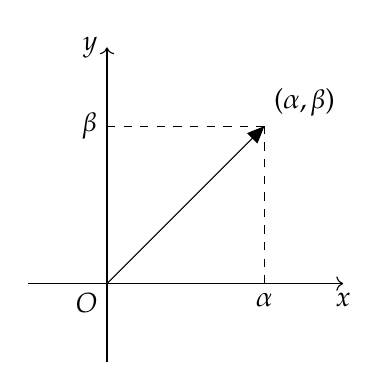
\begin{tikzpicture}[scale=2]%vetor no plano
        \coordinate[label=below left:$O$] (A) at (0,0);
        \coordinate (W) at (1,1);
        %defini\c{c}\~ao das coordenadas dos eixos cartesianos
        \coordinate (F) at (-0.5,0);
        \coordinate (G) at (0,-0.5);
        \coordinate (X) at (1.5,0);
        \coordinate (Y) at (0,1.5);
        % Styles
        \tikzstyle{axes}=[]

        \begin{scope}[style=axes]%constr\'oi os eixos cartesianos
            \draw[->] (F) -- (X) node[below] {$x$} coordinate(x axis);
            \draw[->] (G) -- (Y) node[left] {$y$} coordinate(y axis);
        \end{scope}

        \draw[->,>=triangle 45] (A)--(W)
          node[above right]{$(\alpha, \beta)$};
        \draw[dashed,color=black] let \p1 = (W) in (\x1,0) -- (\x1,\y1)
          node[at start, below]{$\alpha$};
        \draw[dashed,color=black] let \p1 = (W) in (0,\y1) -- (\x1,\y1)
          node[at start, left]{$\beta$};
    \end{tikzpicture}
\end{document}